\chapter{Árvores filogenéticas e relógio molecular}\label{ch:b2:phylogenetic-trees}

Em 1965, dois químicos, Emile Zuckerkandl e Linus Pauling, compararam
as sequências de aminoácidos da hemoglobina de um punhado de vertebrados
e notaram algo que nenhum anatomista poderia ter visto: o número de
diferenças entre duas espécies era proporcional ao tempo decorrido desde
que seus ancestrais tinham se separado, tal como lido nos fósseis. Uma
molécula marcava o tempo. Em uma década, Carl Woese tinha usado um único
gene, o RNA da subunidade menor do ribossomo, para desenhar a árvore de
toda a vida e encontrar nela um terceiro domínio, as arqueias, que nenhum
microscópio tinha distinguido das bactérias. Este capítulo trata da
reconstrução da história a partir da semelhança: o que uma árvore
significa, como ela é construída a partir de caracteres e de distâncias,
como se faz as sequências contarem o tempo, e as armadilhas ---
convergência, taxas desiguais, saturação, ramos longos --- que um leitor
de árvores deve conhecer.

\section{Ler uma árvore}

\begin{definition}[Filogenia, clado, homologia]\label{def:b2:phylogenetic-trees:tree}
\index{filogenia}\index{clado}\index{grupo monofilético}\index{grupo parafilético}\index{grupo polifilético}\index{homologia}\index{analogia}\index{sinapomorfia}
Uma \emph{filogenia} é uma árvore cujas pontas são as espécies (ou os
genes, ou os indivíduos) comparadas, cujos nós internos são seus
ancestrais comuns e cuja raiz é o ancestral mais antigo de todos. Só a
ordem das ramificações carrega a história: os nós podem ser girados
livremente, e só o encaixe importa. Um \emph{clado} ou \emph{grupo
monofilético} é um ancestral com \emph{todos} os seus descendentes (as
aves; os mamíferos; aves e crocodilos juntos); um grupo
\emph{parafilético} é um ancestral com alguns descendentes deixados de
fora (os ``répteis'' sem as aves, os ``peixes'' sem os tetrápodes, os
``procariontes''); um grupo \emph{polifilético} reúne descendentes de
ancestrais diferentes por uma semelhança que eles adquiriram
separadamente (os ``animais de sangue quente''). Um caráter
compartilhado por duas espécies porque seu ancestral o possuía é uma
\emph{homologia} (os ossos da asa do morcego e da nadadeira da baleia);
um caráter que elas adquiriram independentemente é uma \emph{analogia}
ou \emph{homoplasia} (as asas dos morcegos e das aves enquanto asas, os
olhos em câmara dos vertebrados e dos polvos). Só as homologias
registram a história e, entre elas, só os estados \emph{derivados}
compartilhados por um grupo --- suas \emph{sinapomorfias}, na palavra de
Hennig --- definem um clado: as penas definem as aves, e o estado
ancestral ``sem penas'' não define nada.
\end{definition}

\begin{omfigure}
\begin{tikzpicture}[every node/.style={font=\scriptsize}, >=stealth, line width=0.8pt]
  \coordinate (root) at (0,0);
  \coordinate (n1) at (1.2,0.9); \coordinate (n2) at (2.4,1.6); \coordinate (n3) at (3.6,2.3);
  \draw (root) -- (1.4,-1.3) node[right] {mamíferos};
  \draw (root) -- (n1);
  \draw (n1) -- (4.8,-0.1) node[right] {tartarugas};
  \draw (n1) -- (n2);
  \draw (n2) -- (4.8,0.9) node[right] {lagartos, serpentes};
  \draw (n2) -- (n3);
  \draw (n3) -- (4.8,1.9) node[right] {crocodilos};
  \draw (n3) -- (4.8,3.0) node[right] {aves};
  \fill (root) circle (1.6pt); \fill (n1) circle (1.6pt); \fill (n2) circle (1.6pt); \fill (n3) circle (1.6pt);
  \node[left] at (root) {amniotas};
  % groups
  \draw[omThm, thick, rounded corners=6pt] (3.1,1.55) rectangle (6.9,3.4);
  \node[omThm, anchor=south west] at (3.1,3.4) {arcossauros: monofiléticos};
  \draw[omExo!80!black, thick, dashed, rounded corners=6pt] (2.2,-0.5) -- (2.2,2.2) -- (7.1,2.2) -- (7.1,-0.5) -- cycle;
  \node[omExo!80!black, anchor=north east] at (7.1,-0.55) {``répteis'' sem as aves: parafiléticos};
  \node[anchor=west, align=left, text width=4.2cm] at (7.9,1.3) {sinapomorfias:\\ $\bullet$ ovo amniótico (todos)\\ $\bullet$ abertura anterorbital no crânio (arcossauros)\\ $\bullet$ penas (aves)};
\end{tikzpicture}

{\small Ler uma árvore. As aves se aninham dentro dos répteis: os
crocodilos são mais próximos das aves que dos lagartos. O grupo
nomeado ``répteis'' é um ancestral do qual foi removida uma linhagem de
descendentes --- um grado parafilético, e não um \omterm{def:b2:phylogenetic-trees:tree}{clado}.}
\end{omfigure}

\begin{omfigure}
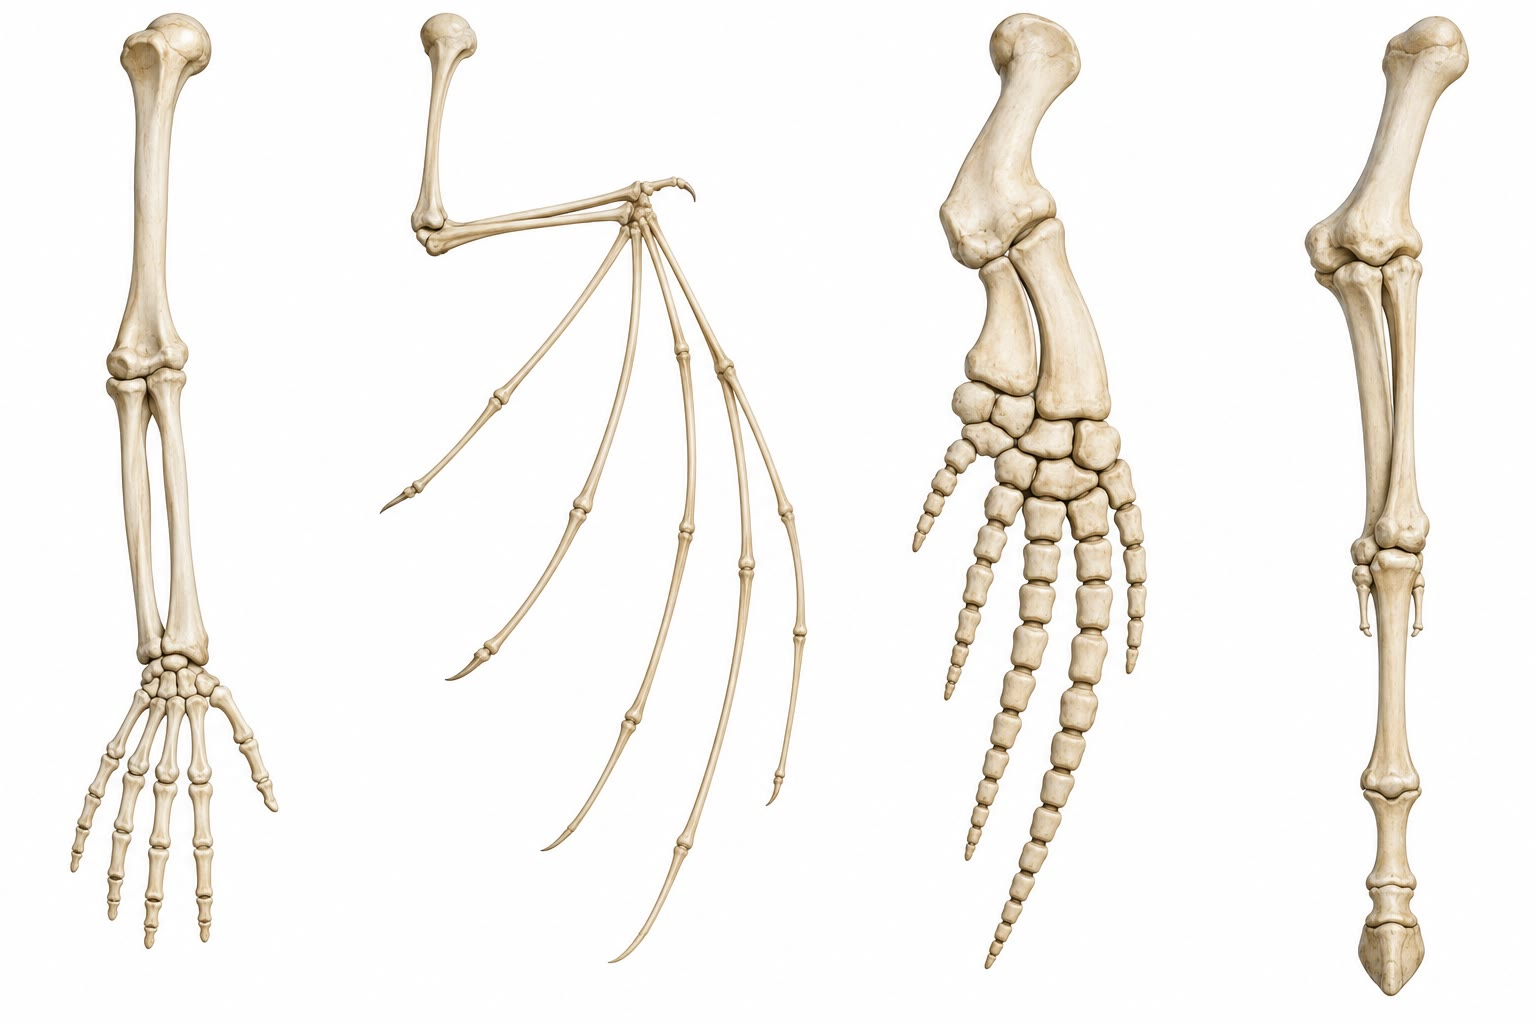
\includegraphics[width=0.44\linewidth]{images/book4/ai/b4-24-homologous-forelimbs.jpg}\hspace{0.04\linewidth}
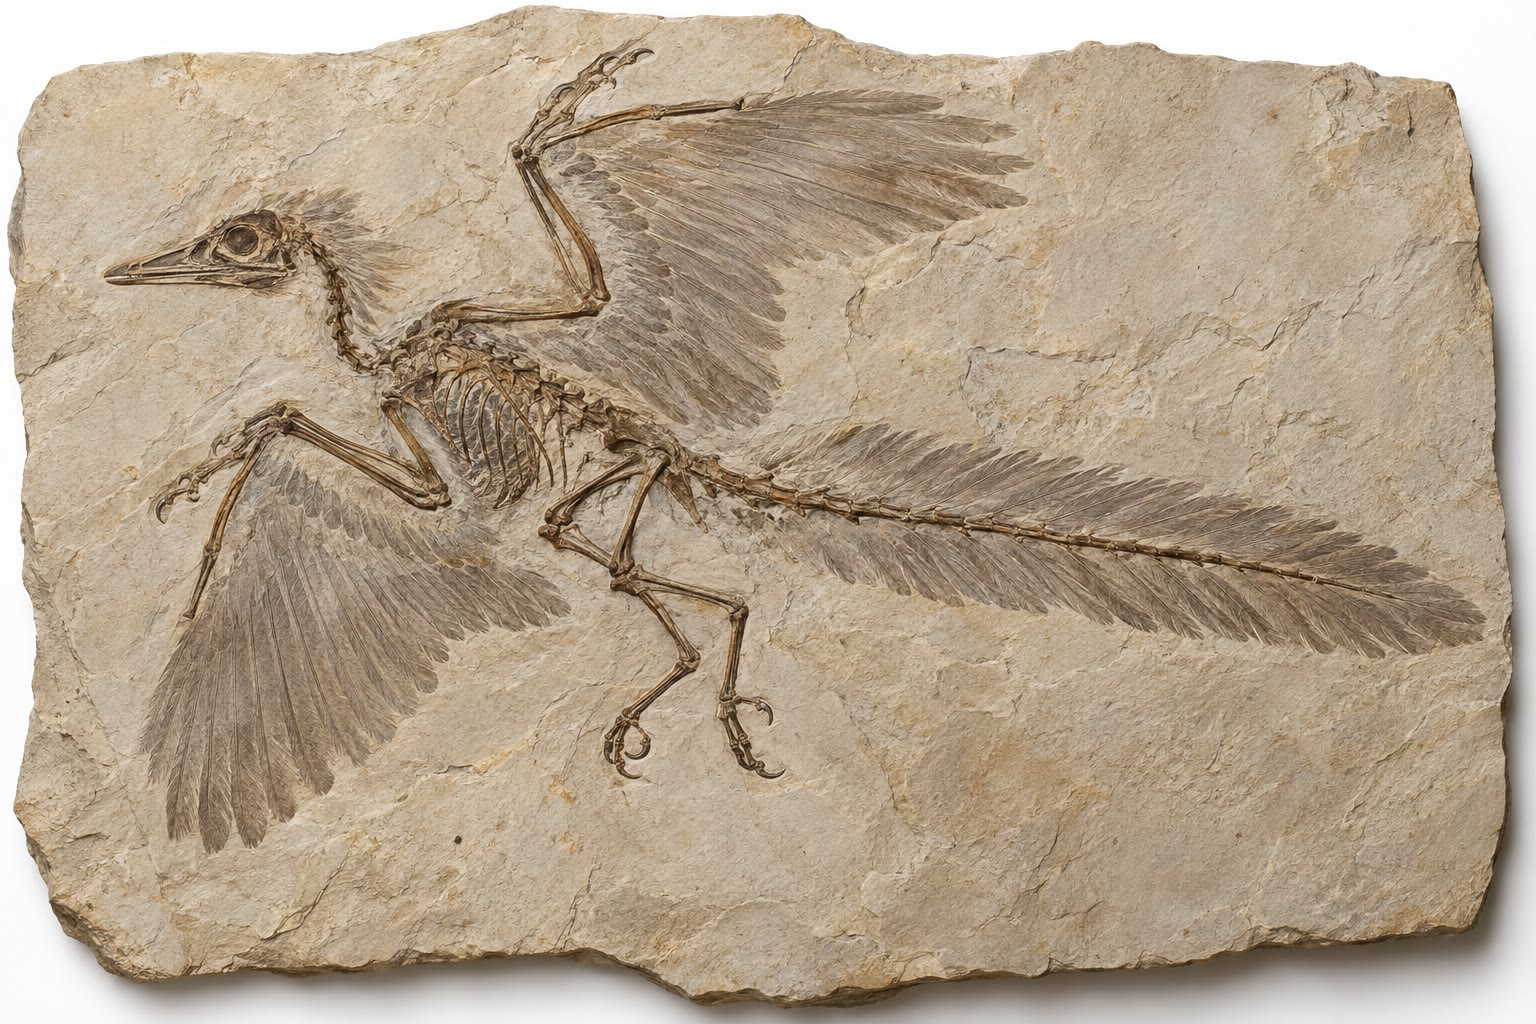
\includegraphics[width=0.44\linewidth]{images/book4/ai/b4-24-archaeopteryx.jpg}

{\small A \omterm{def:b2:phylogenetic-trees:tree}{homologia} e seu registro. À esquerda: os mesmos ossos ---
úmero, rádio e ulna, punho, cinco dedos --- num braço, numa asa, numa
nadadeira e numa pata. À direita: \emph{Archaeopteryx}, com os dentes,
os dedos com garras e a longa cauda óssea de um pequeno dinossauro e as
penas de uma ave.}
\end{omfigure}

\section{Construir árvores a partir de caracteres}

\begin{method}[Parcimônia]\label{meth:b2:phylogenetic-trees:parsimony}
\index{parcimônia}\index{grupo externo}\index{bootstrap}
Codifique os caracteres (estados morfológicos ou posições de sequências
alinhadas) para cada táxon. Para cada árvore possível, conte o número
mínimo de mudanças de caráter necessárias para explicar os dados sobre
ela; a árvore mais parcimoniosa é a que precisa de menos. Enraíze a
árvore com um \emph{\omterm{meth:b2:phylogenetic-trees:parsimony}{grupo externo}}, um táxon que sabidamente está fora do
grupo estudado. Como o número de árvores não enraizadas para $n$ táxons é $1\cdot 3\cdot
5\cdots(2n - 5)$ --- três para quatro táxons, $2\times 10^{6}$ para
dez, $10^{20}$ para vinte ---, a busca só é exaustiva para conjuntos
pequenos, e heurística além deles. A confiança é medida pelo
\emph{bootstrap}: reamostre os caracteres com reposição mil vezes,
reconstrua a árvore a cada vez e registre com que frequência cada \omterm{def:b2:phylogenetic-trees:tree}{clado}
reaparece; um \omterm{def:b2:phylogenetic-trees:tree}{clado} encontrado em \qty{95}{\%} das reamostragens é bem
sustentado, e um encontrado na metade não é.
\end{method}

\begin{example}[Quatro táxons, cinco sítios]\label{ex:b2:phylogenetic-trees:parsimony}
Sequências $A = \mathrm{AAGCT}$, $B = \mathrm{AAGCC}$, $C =
\mathrm{GGACT}$, $D = \mathrm{GGATC}$. Na árvore $((A,B),(C,D))$, os
sítios 1, 2 e 3 mudam uma vez cada um (no ramo interno), o sítio 4
uma vez ($\mathrm{C}\to\mathrm{T}$ em $D$) e o sítio 5 duas vezes
($\mathrm{T}\to\mathrm{C}$ em $B$ e em $D$): seis passos. Em
$((A,C),(B,D))$, os sítios 1--3 precisam de duas mudanças cada um, e os
sítios 4 e 5 de uma cada um: oito. Em $((A,D),(B,C))$: nove. A primeira
árvore é a mais parcimoniosa, por dois passos; os três sítios que a
sustentam são suas \omterm{def:b2:phylogenetic-trees:tree}{sinapomorfias}, e o sítio 5 é uma homoplasia sobre ela
--- a mesma mudança ocorrendo duas vezes, algo corriqueiro em todo
conjunto de dados real.
\end{example}

\begin{omfigure}
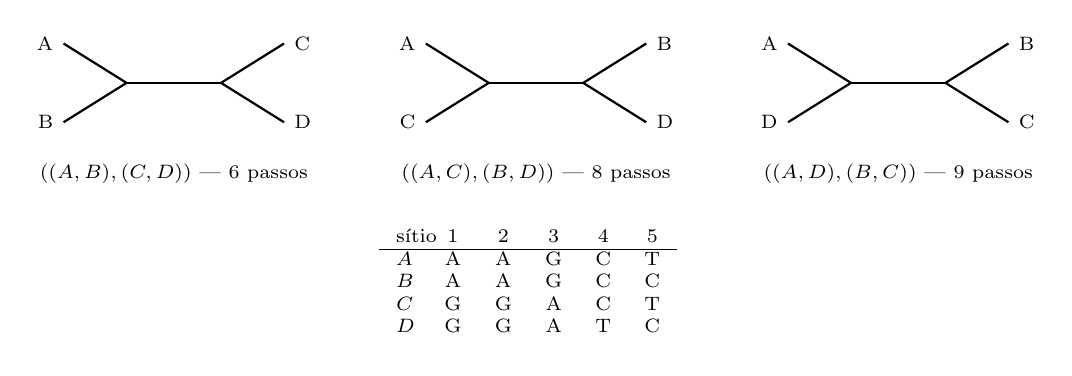
\begin{tikzpicture}[every node/.style={font=\scriptsize}, line width=0.8pt]
  \foreach \x/\a/\b/\c/\d/\steps/\lab in {0/A/B/C/D/6/{$((A,B),(C,D))$ --- 6 passos}, 4.6/A/C/B/D/8/{$((A,C),(B,D))$ --- 8 passos}, 9.2/A/D/B/C/9/{$((A,D),(B,C))$ --- 9 passos}} {
    \begin{scope}[xshift=\x cm]
      \draw (0,1.6) node[left] {\a} -- (0.8,1.1) -- (0,0.6) node[left] {\b};
      \draw (0.8,1.1) -- (2.0,1.1);
      \draw (2.8,1.6) node[right] {\c} -- (2.0,1.1) -- (2.8,0.6) node[right] {\d};
      \node[anchor=north] at (1.4,0.2) {\lab};
    \end{scope}
  }
  \node[anchor=north] at (5.9,-0.6) {\begin{tabular}{l@{\ }ccccc} sítio & 1 & 2 & 3 & 4 & 5 \\ \hline $A$ & A & A & G & C & T \\ $B$ & A & A & G & C & C \\ $C$ & G & G & A & C & T \\ $D$ & G & G & A & T & C \end{tabular}};
\end{tikzpicture}

{\small As três árvores não enraizadas para quatro táxons, avaliadas
com o alinhamento de cinco sítios abaixo delas. Os sítios 1--3 mudam uma
vez na primeira árvore e duas vezes nas outras; o sítio 4 varia em um único táxon
e não consegue decidir, ao passo que o sítio 5 agrupa $A$ com $C$ e assim
favorece a terceira árvore contra elas.}
\end{omfigure}

\section{Construir árvores a partir de distâncias}

\begin{method}[Agrupamento por distância: UPGMA]\label{meth:b2:phylogenetic-trees:upgma}
\index{UPGMA}\index{agrupamento de vizinhos}\index{matriz de distâncias}
A partir das distâncias par a par entre $n$ táxons (diferenças por
sítio, corrigidas como abaixo), junte o par mais próximo num
agrupamento situado num nó de altura igual à metade de sua distância;
substitua o par pelo agrupamento, cuja distância a cada um dos outros
táxons é a média das distâncias de seus membros; repita até restar um
único agrupamento. O resultado é uma árvore enraizada com todas as pontas
na mesma altura --- o método supõe uma taxa de mudança constante em
todos os ramos, um \omterm{thm:b2:phylogenetic-trees:clock}{relógio molecular}. Quando as taxas diferem entre
linhagens, o método agrupa as linhagens de evolução rápida,
qualquer que seja sua história; o \emph{\omterm{meth:b2:phylogenetic-trees:upgma}{agrupamento de vizinhos}}
(\textit{neighbor joining}), que a cada passo junta o par cuja união
mais encurta a árvore inteira, não supõe relógio e é o método rápido
padrão para grandes conjuntos de dados.
\end{method}

\begin{example}[UPGMA]\label{ex:b2:phylogenetic-trees:upgma}
Distâncias (em diferenças por cem sítios): $AB = 4$, $AC = 8$,
$AD = 10$, $BC = 8$, $BD = 10$, $CD = 6$. Junte $A$ e $B$ na altura 2;
depois $d(AB, C) = 8$, $d(AB, D) = 10$, $d(C,D) = 6$: junte $C$ e $D$ na
altura 3; por fim $d(AB, CD) = (8 + 10 + 8 + 10)/4 = 9$: junte os
dois agrupamentos na altura $4.5$. A árvore é $((A,B),(C,D))$ e, se
a taxa for de $10^{-9}$ substituições por sítio por ano, a raiz tem
$0.045/10^{-9} = 45$ milhões de anos.
\end{example}

\begin{omfigure}
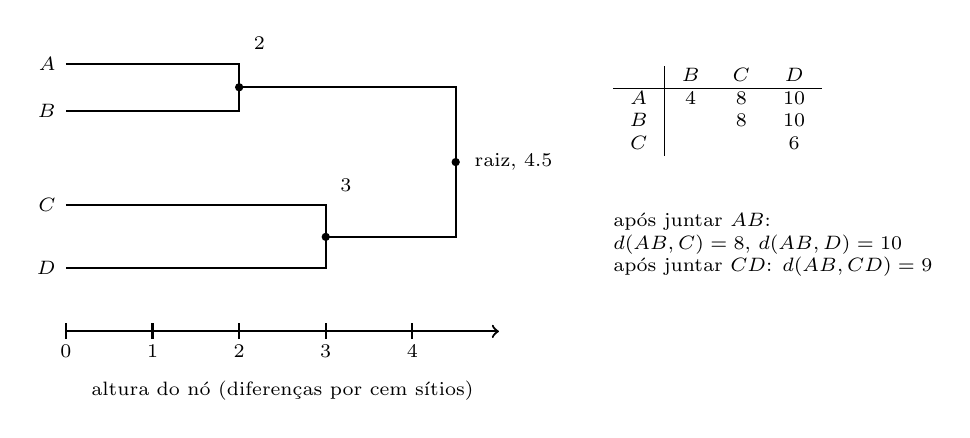
\begin{tikzpicture}[every node/.style={font=\scriptsize}, line width=0.8pt, x=1.1cm]
  \draw[->] (0,-0.4) -- (5,-0.4); \foreach \h in {0,1,2,3,4} \draw (\h,-0.5) -- (\h,-0.3) node[below=4pt] {\h};
  \node[anchor=north] at (2.5,-0.9) {altura do nó (diferenças por cem sítios)};
  % A,B join at 2, C,D at 3, root at 4.5 ; draw as rooted tree, root on the right
  \draw (0,3.0) node[left] {$A$} -- (2,3.0) -- (2,2.4) -- (0,2.4) node[left] {$B$};
  \draw (0,1.2) node[left] {$C$} -- (3,1.2) -- (3,0.4) -- (0,0.4) node[left] {$D$};
  \draw (2,2.7) -- (4.5,2.7) -- (4.5,0.8) -- (3,0.8);
  \fill (2,2.7) circle (1.5pt); \fill (3,0.8) circle (1.5pt); \fill (4.5,1.75) circle (1.5pt);
  \node[anchor=west] at (4.6,1.75) {raiz, 4.5};
  \node[anchor=south west] at (2.05,3.05) {2};
  \node[anchor=south west] at (3.05,1.25) {3};
  \node[anchor=west, align=left] at (6.2,2.4) {\begin{tabular}{c|ccc} & $B$ & $C$ & $D$ \\ \hline $A$ & 4 & 8 & 10 \\ $B$ & & 8 & 10 \\ $C$ & & & 6 \end{tabular}};
  \node[anchor=west, align=left] at (6.2,0.7) {após juntar $AB$:\\ $d(AB,C) = 8$, $d(AB,D) = 10$\\ após juntar $CD$: $d(AB,CD) = 9$};
\end{tikzpicture}

{\small UPGMA com quatro táxons. Cada nó fica na metade da distância
entre os agrupamentos que ele junta; todas as pontas terminam na altura
zero, como exige um relógio.}
\end{omfigure}

\section{O relógio molecular}

\begin{theorem}[As substituições como processo de Poisson e a correção para substituições múltiplas]\label{thm:b2:phylogenetic-trees:clock}
\index{relógio molecular}\index{correção de Jukes--Cantor}\index{saturação}
Se as substituições num sítio ocorrem a uma taxa constante $k$ por ano,
independentemente de um sítio para outro, o número que se acumula ao
longo de uma linhagem num tempo $t$ segue uma lei de Poisson de média
$kt$, e o número esperado que separa duas linhagens que divergiram há
$t$ anos é
\[
d = 2kt
\]
substituições por sítio --- o \emph{\omterm{thm:b2:phylogenetic-trees:clock}{relógio molecular}}. A proporção
observada $p$ de sítios que diferem é menor que $d$, porque um sítio
atingido duas vezes pode voltar à sua base original ou coincidir por
acaso; com quatro bases mudando a taxas iguais,
\[
p = \tfrac{3}{4}\bigl(1 - e^{-4d/3}\bigr), \qquad
d = -\tfrac{3}{4}\ln\bigl(1 - \tfrac{4}{3}p\bigr),
\]
a correção de \emph{Jukes--Cantor}. À medida que $d$ cresce, $p$ satura
em $3/4$ --- duas sequências aleatórias coincidem em um quarto de seus
sítios --- e, além de $p \approx 0.5$, a correção amplia todo erro de
amostragem: um gene que mudou tanto deixou de marcar o tempo. Os genes
lentos (RNA ribossômico, histonas) datam os ramos profundos; os rápidos
(DNA mitocondrial, íntrons), os recentes.
\end{theorem}
\begin{proof}
Seja $q(t)$ a probabilidade de que um sítio ainda tenha sua base
original após um tempo $t$. Ela é perdida à taxa $k$ e recuperada, a
partir de qualquer uma das três outras bases, à taxa $k/3$:
$\mathrm{d}q/\mathrm{d}t = -kq + \tfrac{k}{3}(1 - q) = \tfrac{k}{3} -
\tfrac{4k}{3}q$, cuja solução com $q(0) = 1$ é $q = \tfrac14 +
\tfrac34 e^{-4kt/3}$. Duas linhagens separadas por um tempo total $2t$ ---
por simetria, o mesmo que uma linhagem evoluindo durante $2t$ ---
coincidem num sítio com probabilidade $\tfrac14 + \tfrac34 e^{-4d/3}$, em que $d =
2kt$, logo $p = 1 - q = \tfrac34(1 - e^{-4d/3})$; invertendo, obtém-se a
correção. A contagem de Poisson decorre de eventos constantes e
independentes, como na física do decaimento radioativo, e seu
desvio-padrão $\sqrt{kt}$ fixa a precisão de qualquer data: um gene de $L$
sítios com $dL$ substituições observadas data uma divergência com uma
precisão relativa de cerca de $1/\sqrt{dL}$.
\end{proof}
\begin{proof}[Evidências]
Zuckerkandl e Pauling (1965) constataram que as diferenças entre as
hemoglobinas do cavalo, do ser humano, da vaca e de outros eram
proporcionais às idades fósseis de suas separações, e propuseram o
relógio. Fitch e Margoliash (1967) construíram uma árvore de vinte
espécies apenas a partir do citocromo
$c$ e recuperaram, a partir de uma única proteína, os agrupamentos
clássicos dos vertebrados, dos insetos e dos fungos. O teste decisivo do
método foi a \omterm{def:b2:phylogenetic-trees:tree}{filogenia} experimental de Hillis e colaboradores (1992):
eles propagaram o bacteriófago T7 por uma série conhecida e ramificada
de oito linhagens sob um mutagênico, sequenciaram os produtos e deram as
sequências às cegas aos métodos de construção de árvores --- os métodos
de parcimônia, de distância e de verossimilhança recuperaram todos a
árvore verdadeira, e a parcimônia reconstruiu as sequências ancestrais
com mais de \qty{98}{\%} de exatidão.
\end{proof}

\begin{omfigure}
\begin{tikzpicture}
\begin{axis}[
  width=0.7\linewidth, height=5.4cm,
  axis x line=bottom, axis y line=left,
  xmin=0, xmax=2.5, ymin=0, ymax=1.05,
  xlabel={substituições reais por sítio, $d$}, ylabel={diferenças observadas, $p$},
  xlabel style={font=\small, at={(axis description cs:0.5,-0.13)}, anchor=north},
  ylabel style={font=\small},
  tick label style={font=\small}, ytick={0,0.25,0.5,0.75,1},
  legend style={font=\scriptsize, at={(0.97,0.35)}, anchor=east, draw=none},
  clip=false,
]
\addplot[very thick, omDef, domain=0:2.5, samples=80] {0.75*(1-exp(-4*x/3))};
\addlegendentry{$p = \tfrac34(1 - e^{-4d/3})$}
\addplot[thick, gray, dashed, domain=0:1.05, samples=2] {x};
\addlegendentry{$p = d$: sem substituições múltiplas}
\draw[dotted, gray] (axis cs:0,0.75) -- (axis cs:2.5,0.75); \node[font=\scriptsize, anchor=south east] at (axis cs:2.5,0.75) {saturação, $p = 3/4$};
\draw[<->, omThm, thick] (axis cs:0.383,0.30) -- (axis cs:0.383,0.383); \node[font=\scriptsize, omThm, anchor=west] at (axis cs:0.5,0.22) {$p = 0.30$ significa $d = 0.38$};
\end{axis}
\end{tikzpicture}

{\small Substituições múltiplas. A fração observada de sítios diferentes
sobe com o número real de substituições e depois satura; um $p$ bruto
subestima todas as distâncias e comprime os ramos profundos de uma
árvore.}
\end{omfigure}

\begin{proposition}[Armadilhas do relógio e das árvores]\label{prop:b2:phylogenetic-trees:pitfalls}
\index{atração de ramos longos}\index{heterogeneidade de taxas}\index{separação incompleta de linhagens}\index{verossimilhança (filogenética)}
O relógio é apenas aproximadamente constante: as taxas diferem entre
genes num fator de cem (conforme a função --- a histona H4 mudou dois
resíduos em um bilhão de anos, os fibrinopeptídeos mudam a cada poucos
milhões), entre sítios de um mesmo gene (as terceiras posições dos
códons, os íntrons e as alças mudam mais depressa) e entre linhagens (o
relógio dos roedores anda mais depressa que o dos primatas, com suas
gerações mais curtas e suas taxas metabólicas mais altas). Todo relógio
precisa, portanto, de uma \emph{calibração} por um fóssil ou por um
evento geológico datado, e as datas carregam o erro de Poisson acima e o
da própria calibração. As árvores têm suas próprias armadilhas.
\emph{\omterm{prop:b2:phylogenetic-trees:pitfalls}{Atração de ramos longos}}: duas linhagens que mudaram muito cada uma
compartilham muitos sítios por acaso, e a parcimônia as junta qualquer
que seja sua história --- o remédio é uma amostragem mais densa, que
quebre os ramos, e um método que modele as taxas. A \emph{convergência}
produz falsas \omterm{def:b2:phylogenetic-trees:tree}{sinapomorfias}. \emph{\omterm{prop:b2:phylogenetic-trees:pitfalls}{Separação incompleta de linhagens}}: a
árvore de um gene não é necessariamente a árvore das espécies quando as
especiações se sucedem rapidamente, porque o polimorfismo ancestral se
distribui de modo diferente em cada descendente
--- por isso uma árvore de espécies é construída a partir de muitos
genes, e não de um só. E nos procariontes, onde os genes se deslocam
lateralmente (\cref{ch:b2:genome-diversification}), genes diferentes
contam histórias diferentes, e a história é uma rede atravessada por
uma árvore de genes ribossômicos. A prática moderna substitui a
parcimônia e a distância pela \emph{verossimilhança}: dado um modelo de
substituição (as taxas de cada mudança, sua variação entre sítios),
calcula-se a probabilidade das sequências observadas em cada árvore com
seus comprimentos de ramos e escolhe-se a árvore que torna os dados mais
prováveis; sua forma bayesiana fornece diretamente uma probabilidade
para cada \omterm{def:b2:phylogenetic-trees:tree}{clado}. O volume do Ano 3 apresenta os métodos; aqui basta
saber que toda árvore é uma hipótese com um suporte medido, e não um
fato.
\end{proposition}
\begin{proof}[Evidências]
Woese e Fox (1977) compararam o RNA ribossômico da subunidade menor de
diversos procariontes e constataram que os metanogênicos estão tão
distantes das bactérias quanto ambos estão dos eucariontes: os três
domínios, confirmados desde então por todos os genes da maquinaria de
transcrição e de tradução, e invisíveis para a morfologia. As mesmas
árvores ribossômicas, lidas ingenuamente, colocavam os microsporídios, de
evolução rápida, na base dos eucariontes; genes de taxas mais lentas, e
modelos que levam em conta a variação das taxas, os transferiram para os
fungos, onde é seu lugar --- um caso clássico de \omterm{prop:b2:phylogenetic-trees:pitfalls}{atração de ramos longos}
detectada e corrigida.
\end{proof}

\begin{omfigure}
\begin{tikzpicture}[every node/.style={font=\scriptsize}, line width=0.8pt]
  \node[anchor=south] at (1.5,2.6) {árvore verdadeira};
  \draw (0,2.2) node[left] {$A$} -- (0.8,1.6) -- (0,1.0) node[left] {$B$};
  \draw (0.8,1.6) -- (1.6,1.6);
  \draw[very thick, omThm] (1.6,1.6) -- (3.4,2.4) node[right] {$C$ (rápida)};
  \draw[very thick, omThm] (0.8,1.6) -- (0.8,0.2) -- (2.6,0.2) node[right] {$D$ (rápida)};
  \draw (1.6,1.6) -- (2.4,1.0) node[right] {$E$};
  \begin{scope}[xshift=7cm]
    \node[anchor=south] at (1.5,2.6) {árvore que a parcimônia encontra};
    \draw (0,2.2) node[left] {$A$} -- (0.8,1.6) -- (0,1.0) node[left] {$B$};
    \draw (0.8,1.6) -- (1.6,1.6);
    \draw (1.6,1.6) -- (2.4,1.9) node[right] {$E$};
    \draw[very thick, omThm] (1.6,1.6) -- (2.2,1.0) -- (3.4,1.3) node[right] {$C$};
    \draw[very thick, omThm] (2.2,1.0) -- (3.0,0.2) node[right] {$D$};
  \end{scope}
  \node[align=center, text width=7cm] at (5.6,-1.1) {$C$ e $D$ mudaram, cada uma, em muitos sítios; em um quarto deles, agora coincidem por acaso, mais do que qualquer sinapomorfia verdadeira as liga a seus parentes reais};
\end{tikzpicture}

{\small \omterm{prop:b2:phylogenetic-trees:pitfalls}{Atração de ramos longos}. Duas linhagens que evoluíram mais
depressa são juntadas pelas coincidências fortuitas que suas muitas
mudanças produzem, e a parcimônia faz delas grupos-irmãos.}
\end{omfigure}

\begin{example}[Datar com um fóssil]\label{ex:b2:phylogenetic-trees:dating}
Um gene de \num{1000} sítios difere em \qty{10}{\%} deles entre a vaca e
a baleia, cujo ancestral comum os fósseis situam há 60 milhões de anos.
Corrigido, $d = -0.75\ln(1 - 0.133) = 0.107$; a taxa é $k
= d/2t = 0.107/(1.2\times 10^{8}) = 9\times 10^{-10}$ por sítio por
ano. O mesmo gene difere em \qty{6}{\%} entre a baleia e o hipopótamo:
$d = 0.0625$, $t = d/2k = 35$ milhões de anos, com cerca de $\pm
\qty{13}{\%}$ vindos da contagem de Poisson de 62 substituições e uma
incerteza adicional vinda da data fóssil. O resultado molecular de que
as baleias são as parentes vivas mais próximas dos hipopótamos, obtido
assim nos anos 1990 contra todas as árvores anatômicas, foi confirmado
pela descoberta de baleias primitivas com o osso do tornozelo semelhante
ao do hipopótamo que tinha sido previsto --- o relógio não apenas data;
ele prevê o que as rochas devem conter.
\end{example}

\section{Exercícios}

\begin{exercise}[$\star$]\label{exo:b2:phylogenetic-trees:1}
Defina \omterm{def:b2:phylogenetic-trees:tree}{homologia}, \omterm{def:b2:phylogenetic-trees:tree}{analogia} e \omterm{def:b2:phylogenetic-trees:tree}{sinapomorfia}, com um exemplo de cada entre
os membros, as asas e os olhos dos vertebrados.
\end{exercise}

\begin{exercise}[$\star$]\label{exo:b2:phylogenetic-trees:2}
Classifique como monofilético, parafilético ou polifilético: as aves;
os répteis (sem as aves); os peixes (sem os tetrápodes); os vertebrados
voadores; os mamíferos; os procariontes.
\end{exercise}

\begin{exercise}[$\star$]\label{exo:b2:phylogenetic-trees:3}
Na árvore $(\text{mamíferos},(\text{tartarugas},(\text{lagartos},
(\text{crocodilos},\text{aves}))))$, nomeie o grupo-irmão das
aves, o grupo-irmão dos mamíferos e o menor \omterm{def:b2:phylogenetic-trees:tree}{clado} que contém
lagartos e aves. Trocar as posições dos crocodilos e das aves muda a
árvore?
\end{exercise}

\begin{exercise}[$\star$]\label{exo:b2:phylogenetic-trees:4}
Quantas árvores não enraizadas existem para 4, 6 e 10 táxons? Quantas
árvores enraizadas para 4 (cada árvore não enraizada pode ser enraizada
em qualquer um de seus ramos)?
\end{exercise}

\begin{exercise}[$\star\star$]\label{exo:b2:phylogenetic-trees:5}
Sequências $A = \mathrm{CCTAG}$, $B = \mathrm{CCTGG}$, $C =
\mathrm{TTCAG}$, $D = \mathrm{TTCGA}$. Conte os passos em cada uma das
três árvores não enraizadas e dê a mais parcimoniosa. Quais
sítios são homoplásicos nela?
\end{exercise}

\begin{exercise}[$\star\star$]\label{exo:b2:phylogenetic-trees:6}
Distâncias (por cem sítios): $AB = 6$, $AC = 14$, $AD = 16$,
$BC = 14$, $BD = 16$, $CD = 10$. Construa a árvore UPGMA com as alturas
de seus nós.
\end{exercise}

\begin{exercise}[$\star\star$]\label{exo:b2:phylogenetic-trees:7}
Corrija $p = 0.05$, $0.30$ e $0.60$ para substituições múltiplas. Por
que o terceiro valor é quase inútil?
\end{exercise}

\begin{exercise}[$\star\star$]\label{exo:b2:phylogenetic-trees:8}
Um gene evolui a $10^{-9}$ substituições por sítio por ano. Duas
espécies diferem em $d = 0.02$: quando se separaram? Que $p$ se
observaria entre duas espécies que se separaram há 500 milhões de anos,
e o que isso implica para datar separações profundas com esse gene?
\end{exercise}

\begin{exercise}[$\star\star$]\label{exo:b2:phylogenetic-trees:9}
Um \omterm{def:b2:phylogenetic-trees:tree}{clado} aparece em \qty{52}{\%} de \num{1000} reamostragens bootstrap;
outro, em \qty{99}{\%}. Interprete ambos. O que você faria a respeito
do primeiro?
\end{exercise}

\begin{exercise}[$\star\star\star$]\label{exo:b2:phylogenetic-trees:10}
Explique a \omterm{prop:b2:phylogenetic-trees:pitfalls}{atração de ramos longos} com o argumento do quarto por acaso
e diga por que acrescentar táxons que quebram os ramos longos ajuda.
\end{exercise}

\begin{exercise}[$\star\star\star$]\label{exo:b2:phylogenetic-trees:11}
O DNA mitocondrial do ser humano e o do chimpanzé diferem em \qty{9}{\%}
dos sítios; a taxa mitocondrial é de cerca de $2\times 10^{-8}$ por
sítio por ano. Date a separação, dê a incerteza de Poisson para um
genoma de \qty{16000}{} sítios e cite duas razões pelas quais a resposta
ainda poderia estar errada por um fator de dois.
\end{exercise}

\begin{exercise}[$\star\star\star$]\label{exo:b2:phylogenetic-trees:12}
``Uma árvore de genes não é uma árvore de espécies.'' Discuta, com a
\omterm{prop:b2:phylogenetic-trees:pitfalls}{separação incompleta de linhagens}, a transferência horizontal e a
\omterm{prop:b2:genome-diversification:duplication}{duplicação gênica}, e diga como, apesar disso, se obtém uma árvore de
espécies.
\end{exercise}

\section{Problema: Datar as baleias}

\begin{problem}[{Problema de fim de semana --- baleia, hipopótamo, vaca,
porco e camelo sequenciados para um gene: a árvore construída por
parcimônia e por distância, o relógio calibrado com um fóssil, cada
separação datada com seu erro de Poisson, e a árvore anatômica
confrontada com a molecular, terminando com o tempo de divergência entre
baleia e hipopótamo e a taxa de substituição do gene}]
\label{pb:b2:phylogenetic-trees:1}
Um gene de \num{1000} sítios é sequenciado na baleia ($W$), no
hipopótamo ($H$), na vaca ($C$), no porco ($P$) e no camelo ($M$, o
\omterm{meth:b2:phylogenetic-trees:parsimony}{grupo externo}). Proporções observadas de sítios diferentes: $WH = 0.06$; $WC = HC = 0.10$; $WP =
HP = CP = 0.12$; todas as distâncias a $M$ valem $0.14$. Os fósseis
situam a separação entre a vaca e a linhagem baleia--hipopótamo há 60
milhões de anos. Seis sítios informativos, com o estado do camelo dado
por último:
\begin{center}
\begin{tabular}{l@{\quad}cccccc}
sítio & 1 & 2 & 3 & 4 & 5 & 6 \\ \hline
$W$ & A & G & T & C & A & G \\
$H$ & A & G & T & C & G & G \\
$C$ & G & A & T & T & G & G \\
$P$ & G & A & C & T & G & A \\
$M$ & G & A & C & T & G & A \\
\end{tabular}
\end{center}

\medskip
\noindent\textbf{Parte I --- Parcimônia.}
\begin{enumerate}
  \item Quais sítios são \omterm{def:b2:phylogenetic-trees:tree}{sinapomorfias} de $\{W, H\}$? E de $\{W, H,
        C\}$? Qual sítio não é informativo, e qual é uma homoplasia
        ou autapomorfia?
  \item Conte os passos dos seis sítios na árvore
        $(M,(P,(C,(W,H))))$.
  \item Conte-os na árvore dos anatomistas $(M,(P,(W,(C,H))))$,
        que coloca o hipopótamo com a vaca entre os artiodáctilos e
        as baleias de fora.
  \item Qual árvore é preferida, e por quantos passos? Por que essa
        margem é fraca, e o que a reforçaria?
  \item O bootstrap dá o \omterm{def:b2:phylogenetic-trees:tree}{clado} $\{W, H\}$ em \qty{83}{\%} das
        reamostragens do gene inteiro. Interprete.
  \item Por que o camelo é usado como \omterm{meth:b2:phylogenetic-trees:parsimony}{grupo externo}, e o que daria
        errado se fosse usado um peixe?
\end{enumerate}

\medskip
\noindent\textbf{Parte II --- Distâncias.}
\begin{enumerate}[resume]
  \item Corrija os quatro valores distintos de $p$ ($0.06$, $0.10$, $0.12$,
        $0.14$) para substituições múltiplas.
  \item Aplique o UPGMA aos cinco táxons com as distâncias corrigidas e
        dê as alturas dos nós.
  \item A árvore de distâncias concorda com a árvore de parcimônia?
  \item Explique por que o UPGMA falharia se a linhagem da baleia
        tivesse evoluído duas vezes mais depressa que as outras.
  \item Calcule o número de substituições que o gene acumulou entre a
        baleia e o hipopótamo, e seu desvio-padrão
        de Poisson.
  \item Dê a precisão relativa de uma data baseada nessa contagem.
\end{enumerate}

\medskip
\noindent\textbf{Parte III --- O relógio.}
\begin{enumerate}[resume]
  \item Calibre: a partir da distância vaca--(baleia, hipopótamo) e do
        fóssil de 60 milhões de anos, calcule a taxa $k$ por sítio por
        ano.
  \item Date a separação baleia--hipopótamo.
  \item Date a separação do porco e a do camelo.
  \item Dê a data baleia--hipopótamo com sua incerteza de Poisson.
  \item A calibração fóssil é ela própria incerta em $\pm 5$
        milhões de anos. Propague essa incerteza para a data baleia--hipopótamo.
  \item Um outro gene, mais rápido, dá $p = 0.45$ entre a baleia e o
        camelo. Corrija esse valor e comente sua confiabilidade para essa
        separação.
\end{enumerate}

\medskip
\noindent\textbf{Parte IV --- Confronto.}
\begin{enumerate}[resume]
  \item A árvore dos anatomistas se apoia no astrágalo em dupla polia,
        compartilhado pela vaca, pelo porco, pelo hipopótamo e pelo
        camelo, mas não pelas baleias atuais, que não têm membros
        posteriores. Explique por que um caráter perdido não pode contar
        contra o \omterm{def:b2:phylogenetic-trees:tree}{clado} baleia--hipopótamo.
  \item Baleias fósseis com membros posteriores foram encontradas em
        2001; seu astrágalo tem a dupla polia. O que isso faz com o
        argumento?
  \item Se as baleias estão dentro dos artiodáctilos, o grupo
        ``artiodáctilos sem as baleias'' é monofilético,
        parafilético ou polifilético?
  \item Um segundo gene dá a árvore $(M,(P,(H,(W,C))))$. Cite duas
        razões pelas quais uma árvore de genes pode diferir da árvore de
        espécies, e diga como decidir.
  \item O genoma mitocondrial da baleia e o do hipopótamo diferem em
        \qty{25}{\%} dos sítios. Corrija esse valor e estime a taxa
        mitocondrial a partir da data encontrada na questão 14.
  \item Por que essa taxa é tão mais alta que a do gene nuclear?
  \item Enuncie o resultado: a árvore, a taxa nuclear $k$ e o tempo de
        divergência baleia--hipopótamo com sua incerteza.
\end{enumerate}
\end{problem}
